\documentclass{article}
\usepackage{graphicx}
\usepackage{amsmath}
\usepackage{wrapfig}

\title{Chaos auf dem Billiardtisch}
\author{Johannes Popp}
\date{Sommerakademie, Olang 2012}

 \begin{document}
 
 \title{Chaos auf dem Billiardtisch}
 \author{Johannes Popp}
 \date{Sommerakademie, Olang 2012}
 \maketitle
 \begin{abstract}
 Es werden drei verschiedene Herangehensweisen von Billiards vorgestellt: Zuerst wird eine einfache mathematische Modellierung des klassisch Billiardtisches betrachtet, weiter werden Grundlagen in der Statistischen Physik mit Billiards verbunden, was zur Einf\"{u}hrung des Lorentz-Gas-Modelles f\"{u}hrt und zum Schluss werden klassische Billards durch Wellen ersetzt und genauer studiert.
 \end{abstract}
 
 \section{Mathematische Modellierung}
 
 F\"{u}r die mathematische Formulierung wird meist eine konvexe Berandung Punkt\-teilchen und Reibungslosigkeit genommen. Dies f\"{u}hrt zur bekannten Regel: Einfallswinkel gleich Ausfallswinkel. Um genauere Aussagen machen zu k\"{o}nnen, werden Poincarr\'{e}-Abbildung im Phasenraum betrachtet. Hier stellen sich verschiedene Muster ein:
 
 
 \begin{enumerate}
 \item Bestimmte Anzahl Punkte $\leftrightarrow$ Periodische Orbits
 \item Invariante Kurven $\leftrightarrow$ Invariante Kurven in Betracht der
 Dynamik
 \item \"{U}briger Raum mit einzelnen Punkten $\leftrightarrow$ Chaotische Bahnen
 \end{enumerate}
 
 
 \begin{wrapfigure}{l}{0.5\textwidth}
 \vspace{-20pt}
 \begin{center}
 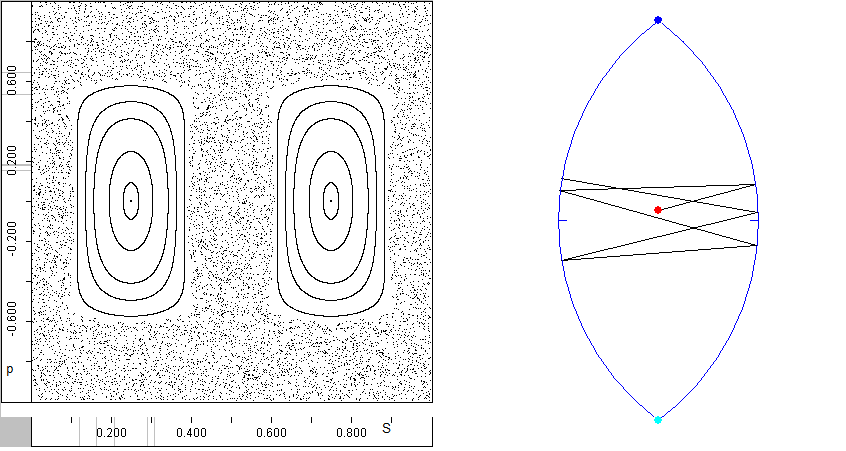
\includegraphics[width=0.5\textwidth]{../citron.jpg}
  \end{center}
  \vspace{-20pt}
  \caption{Zitronenbilliard und das dazugeh\"{o}rige Phasenraumdiagramm}

 \end{wrapfigure}
 
 
 Ein Beispiel, indem alle drei Eigenschaften sich im Phasenraumbild ergeben, ist der Zitronen Billiard (Fig. 1). Der einzige bekannte integrable Billiard ist die Ellipse. Dagegen sind Stadion und Sinaibilliard (Viereck mit Kreis in der Mitte) zwei v\"{o}llig chaotische Billiards. Eine exakte mathematische Modellierung stet noch aus und genauso ein Beweis, dass die Ellipse einzigartig ist in ihrer integrablen Eigenschaft.
 
 \section{Verallgemeinerung, Lorentz-Gas-Modell}
 
 
  \begin{wrapfigure}{r}{0.5\textwidth}
  \vspace{-10pt}
  \begin{center}
  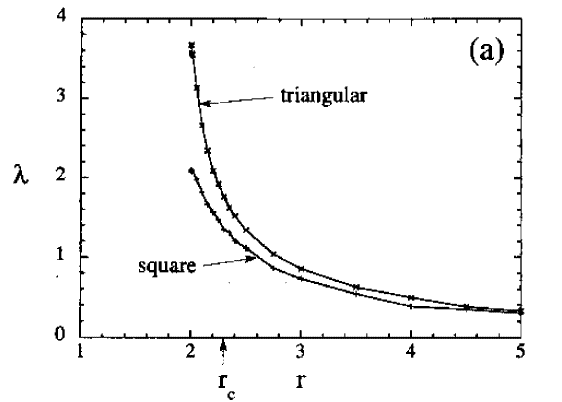
\includegraphics[width=0.5\textwidth]{../LGMstat1.png}
   \end{center}
   \vspace{-10pt}
   \caption{Lypunov-Exponent in Abhängigkeit des Abstandes r der Kreisscheiben mit fixem Radius a}

  \end{wrapfigure}
  
  Mit der Verallgemeinerung werden Billiards mit beliebigen R\"{a}ndern betrachtet. Um den Lyapunovexponenten zu bestimmen wird der zweite fundamentale Operator eingef\"{u}hrt, welcher Ort- und Geschwindigkeitsvariation verbindet. F\"{u}r das Lorentz-Gas-Modell wird daf\"{u}r eine regelm\"{a}ssig Anordnung von Kreisscheiben (Dreieckskristall) betrachtet und der Lyapunov-Exponent berechnet. 
  
  
  F\"{u}r die N\"{a}herung grosser Abst\"{a}nde $r$ ergibt sich der Lyapunov-Exponenten $\lambda \sim ln(r)/r^2$. Mit diesem Modell kann ferner Diffusion und Transport, Druck und Mehrteilchensysteme genauer untersucht werden.
  
  
 \section{Billiards als Wellen}
 
 Die Helmhotzgeichung $(\Delta + k_n^2)\psi(x)=0$ beschreibt mit gegebenen Randbedingungen (Dirichlet oder Neumann) Wellen in Billiards, wobei die Dispersionsrelation $k_n = k_n(\omega)$ festlegt um welche Wellen es sich handelt. Viel beobachtet sind Mikrowellenbilliards; Hier wird ein Wellenleiter in Form eines Billiards auf Eigenfrequenzen untersucht. Interessant ist hierbei der \"{U}bergang zur Quantenmechanik, wo Quantumcorrals betarchtet werden. Um Ausagen \"{u}ber Chaos zu machen muss das Spektrum der Eigenfrequenzen genauer untersucht werden.
 
     \begin{wrapfigure}{l}{0.5\textwidth}

     \begin{center}
     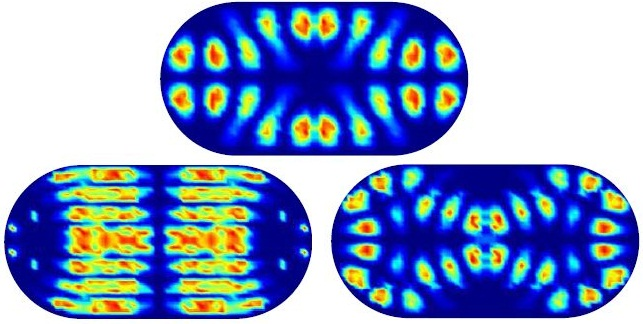
\includegraphics[width=0.45\textwidth]{../Stadium_billiards.jpg}
      \end{center}

      \caption{Mikrowellenbilliards zu verschiedenen Eigenfrequenzen}
     \end{wrapfigure}
 
  \begin{thebibliography}{9}    
  
   \bibitem{ChaosPC}
     H.J. Korsch, H.J. Jodl, T. Hartmann.
     \newblock {\em Chaos: A Program Collection for the PC}.
     \newblock Springer, 2008.
 
   \bibitem{QC}
     H.J. St\"{o}ckmann.
     \newblock {\em Quantum Chaos: An Introduction}.
     \newblock CUP, 1999.
 
   \bibitem{Gaspard}
     P. Gaspard.
     \newblock {\em Chaos, Scattering and Statistical Mechanics}.
     \newblock CUP,1998.
 
 \end{thebibliography}
 \end{document}